\subsection{Salida}
    \begin{figure}[ht]
        \begin{adjustbox}{addcode={
            \begin{minipage}{\width}}{
                \caption{Salida de los tiempos en serie y paralelo}
            \end{minipage}},rotate=360,center}
            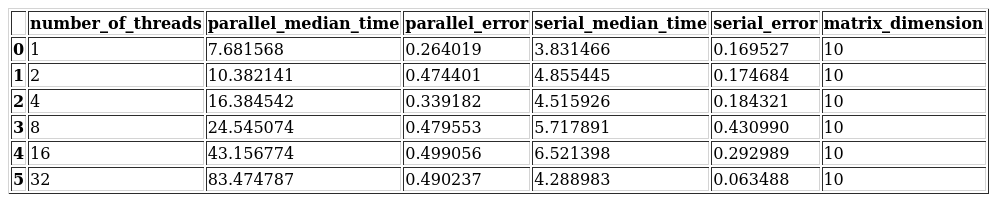
\includegraphics[scale=.6]{amdahl_output_table.png}
        \end{adjustbox}
    \end{figure}
    \FloatBarrier

    De acuerdo a estos datos podemos calcular el speed up maximo, real y teórico.

    \begin{figure}[ht]
        \begin{adjustbox}{addcode={
            \begin{minipage}{\width}}{
                \caption{Speed up real, teorico y maximo segun la cantidad de threads}
            \end{minipage}},rotate=360,center}
            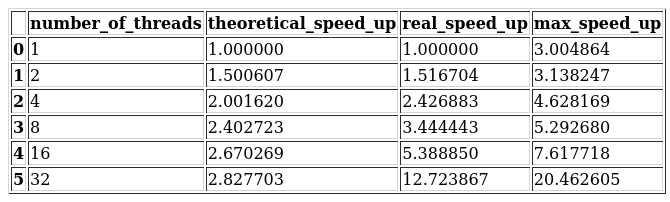
\includegraphics[scale=.6]{amdahl_speed_up_table.png}
        \end{adjustbox}
    \end{figure}
    \FloatBarrier
    \begin{figure}[ht]
        \begin{adjustbox}{addcode={
            \begin{minipage}{\width}}{
                \caption{Grafico}
            \end{minipage}},rotate=360,center}
            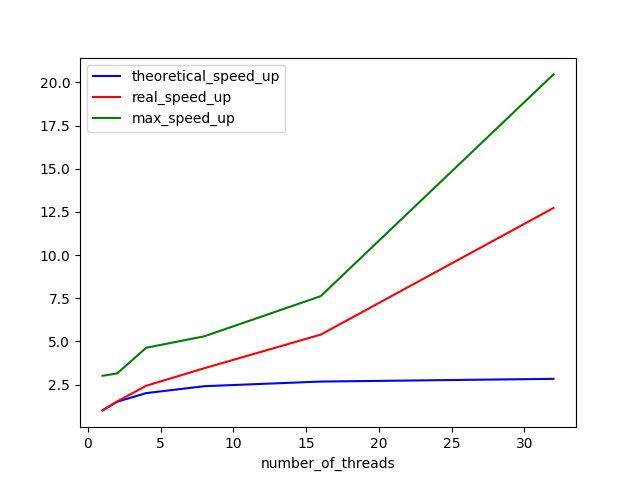
\includegraphics[scale=.6]{amdahl_speed_up.png}
        \end{adjustbox}
    \end{figure}
    \FloatBarrier

    Podemos observar que a medida que aumentan la cantidad de threads aumenta
    el speed up pero en el teorico, una vez que alcanzamos los cuatro threads
    (que es la canitdad maxima de nuestra pc) se mantiene constante. Sin embargo
    el speed up real sigue aumentando y en los 32 threads pega un salto
    considerable. Este resultado es bueno ya que aprovecha la paralelizacion
    para separar el trabajo en los distintos threads.'\